\section{Leggi di controllo}
In questa sezione verranno accennati diversi modelli di controlli utilizzati odiernamente per controllare i quadricotteri, \cite{ZuluAndrew2014ARoC}, \cite{KimJinho2020ACSo}, \cite{PID_vs_LQ}, \cite{G_inf}. Questi si possono classificare in tre categorie come in Figura (\ref{fig:categoriecontrolli}).
\begin{figure}
	\centering
	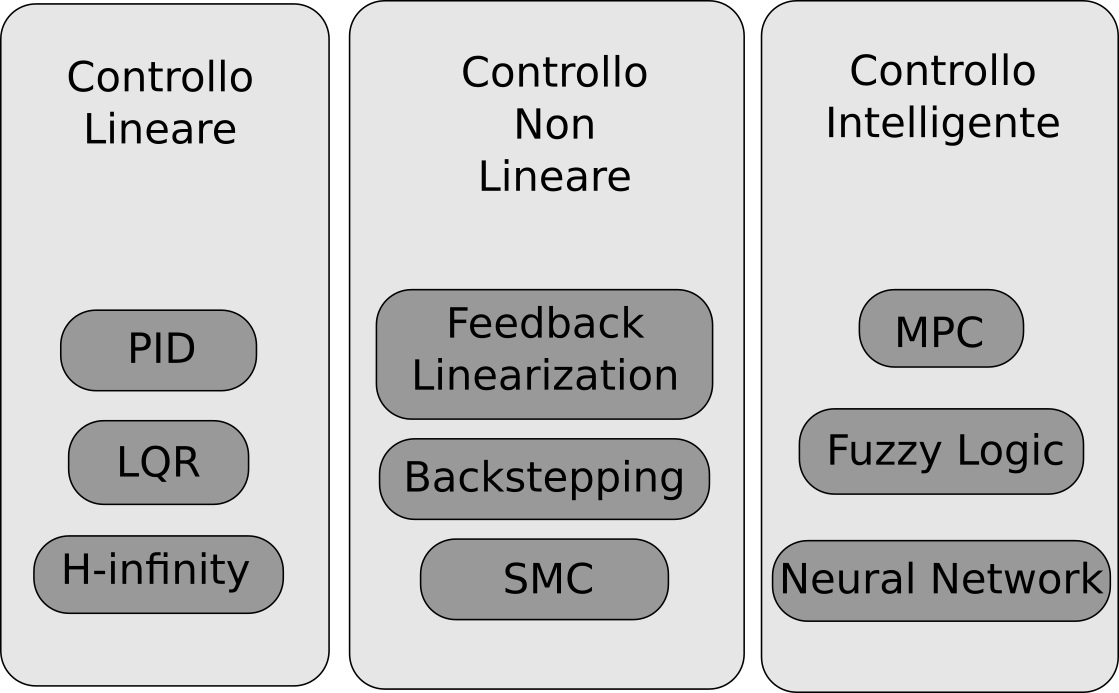
\includegraphics[width=0.6\textwidth]{SistemaQuadrirotore/Figure/Classificazione}
	\caption{Classificazione dei tipi di controllori maggiormente utilizzati \cite{KimJinho2020ACSo}}
	\label{fig:categoriecontrolli}
\end{figure}


\subsection{Controllori Lineari}
\subsubsection{Controllore Proportional-Integral-Derivative Controller (PID)}
Il controllore PID è molto utilizzato in diverse applicazioni, la sua semplicità e facilità di impostazione dei parametri lo rende molto rapido da implementare e relativamente robusto. Inoltre non è necessario avere la misura dello stato completo del sistema da controllare, semplificando eventualmente la determinazione di questo. Il principale problema risiede nella risposta alle eventuali non linearità presenti nel modello del sistema controllato o nella realtà.
Assumendo un errore di misurazione $e(t)$ come la differenza tra il valore atteso $x(t)_{ref}$ e il valore misurato nel sistema $x(t)$ di un qualunque elemento del vettore di stato : $e(t)=x(t)_{ref}-x(t)$. Attraverso la misurazione dell'errore, applicando l'equazione integro differenziale (\ref{eq:SistemaQuadrirotore_PIDErrore}), si determina il comando da attuare sul sistema, \cite{advanced-pid-control}.
\begin{equation}\label{eq:SistemaQuadrirotore_PIDErrore}
	u(t) = k_p e(t) + k_i \int_0^t e(\tau) d\tau + k_d \frac{d e(t)}{d t}
\end{equation}
Il nome del controllore deriva proprio dalla combinazione di questi tre aspetti presi in considerazione per valutare il comando da attuare.
Nell'equazione (\ref{eq:SistemaQuadrirotore_PIDErrore}) sono presenti i tre parametri: $k_p$, $k_i$ e $k_d$.
L'effetto del guadagno proporzionale $k_p$ è quello di ridurre l'errore in modo proporzionale allo stesso. Più l'errore è grande più sarà importante l'intervento del controllore per ridurlo. Un guadagno troppo alto però può provocare un grande superamento del segnale di riferimento causando un overshoot e l'amplificazione delle oscillazioni nella fase di assestamento.
L'effetto $k_i$ è quello ridurre l'errore stazionario terminata la fase di assestamento. Il solo utilizzo della componente proporzionale non è infatti sufficiente per ridurre anche l'errore stazionario, definito come il valore assunto dall'errore trascorso un tempo sufficientemente lungo. Con il solo effetto proporzionale l'errore stazionario si assesta ad un valore finito, il valore integrale dell'errore tende ad aumentare nel tempo se questo on viene annullato, determinando una retroazione integrale che tende a ridurlo.
La derivata dell'errore è invece utile a prevedere il comportamento di questo nel tempo, anticipando l'effetto del proporzionale. Tenendo conto del suo andamento, attraverso il valore di $k_d$, si può ridurre il picco generato da un guadagno alto dell'effetto proporzionale. Questo contributo però va usato con cautela perché amplificare il rumore presente nelle misurazioni.
Il settaggio di questi parametri viene fatta impostando inizialmente solo il valore di $k_p$. Successivamente per ridurre il valore dell'errore stazionario viene aumentato il guadagno $k_i$. Modificando il valore $k_d$ si può ottenere un miglioramento in termini di risposta del sistema, rendendola più stabile. Il processo è iterativo fino ad ottenere una risposta desiderata \cite{advanced-pid-control}.


\begin{figure}
	\centering
	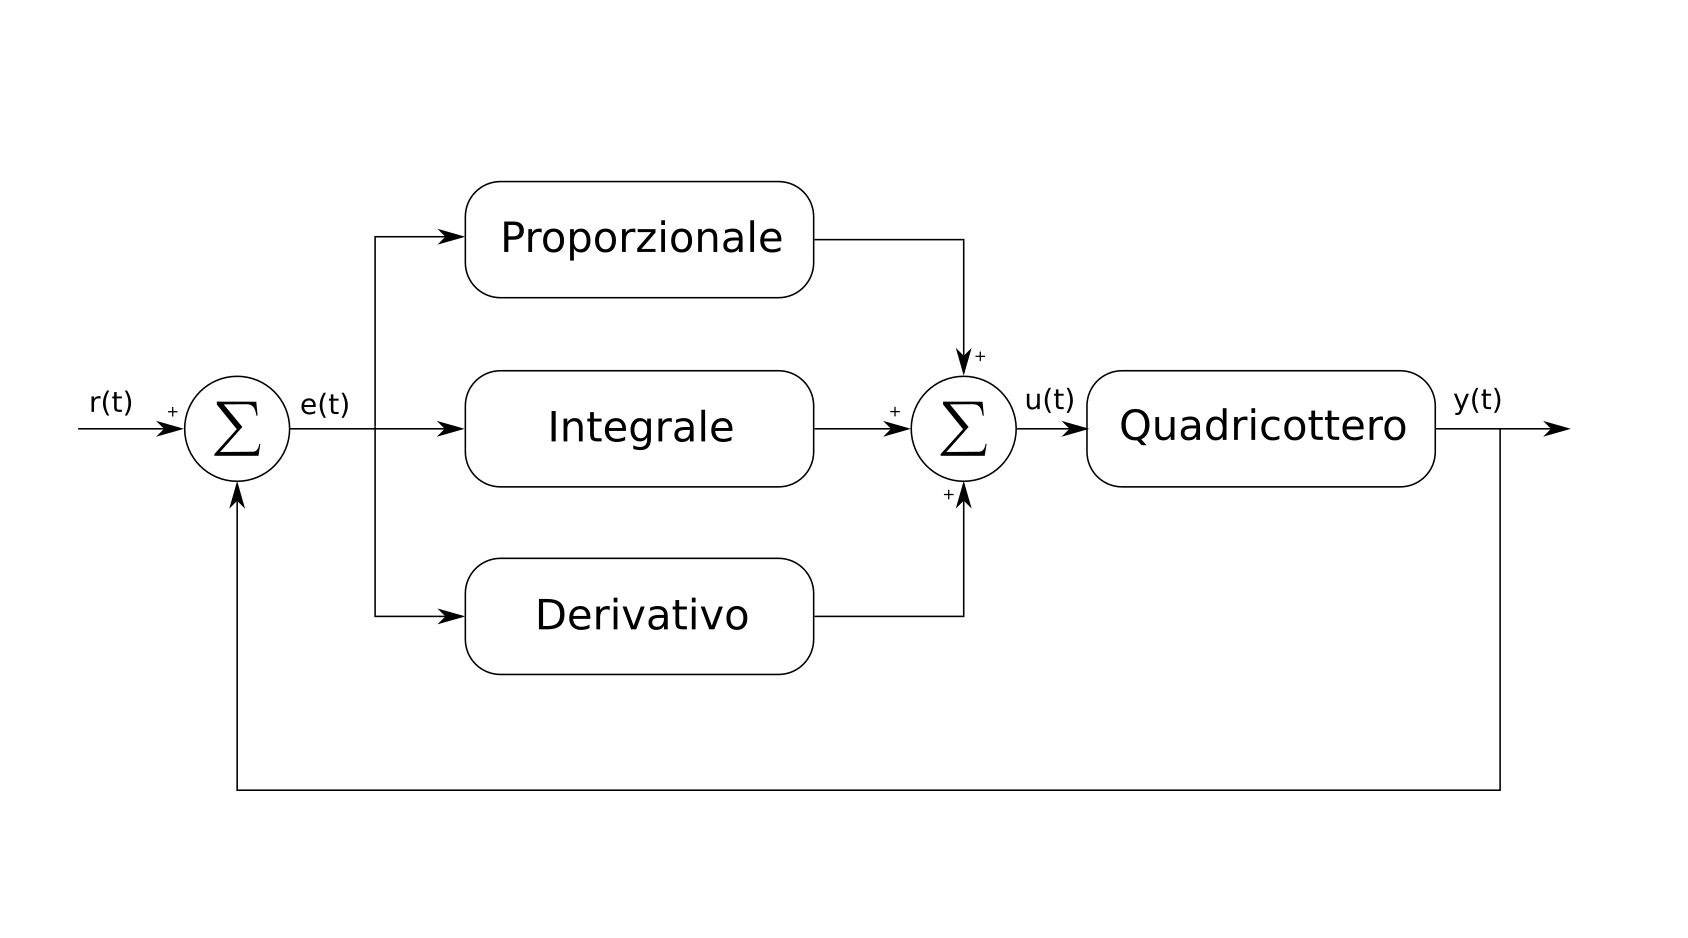
\includegraphics[width=0.6\textwidth]{SistemaQuadrirotore/Figure/PID}
	\caption{Schema di applicazione del controllore PID}
\end{figure}

\subsubsection{Controllore Linear Quadratic Regulator (LQR)}
Con la minimizzazione della funzione di costo espressa nella equazione (\ref{eq:SistemaQuadrirotore_LQRCosto}), si ottiene una matrice di guadagni $\mathbf{K}$ con la quale si applica il controllo in retroazione, Eq. (\ref{eq:SistemaQuadrirotore_K_LQR}), \cite{ParaskevopoulosP.N2002MCE}, \cite{6572698}. A differenza del PID, questo tipo di controllo prevede di avere tutto il vettore di stato a disposizione. Per questo motivo viene accompagnato spesso da un Linear Quadratic Estimator (LQE) ed un filtro di Kalman, con lo scopo di determinare dalle misurazioni dei sensori lo stato completo del sistema da controllare. Il metodo utilizzato per determinare la matrice dei guadagni è un aspetto molto importante, inoltre è necessario modellare in modo molto preciso il sistema controllato per evitare di trovare una soluzione poco soddisfacente. Nel caso si considerino sistemi tempo invarianti la soluzione si può determinare attraverso l'equazione di Ricatti (\ref{eq:SistemaQuadrirotore_Ricatti}), da qui si ottiene la soluzione (\ref{eq:SistemaQuadrirotore_Ricatti_sol}) \cite{baseTesi}. Questo tipo di controllo può essere specializzato per ottenere una soluzione ottima di risparmio della batteria attraverso la scelta delle matrici $\mathbf{Q}$ ed $\mathbf{R}$ \cite{KoksalN2018ALQA}. Gli elementi delle due matrici rappresentano il contributo nella funzione di costo del corrispettivo elemento del vettore di stato o di comando. Più precisamente, aumentando i valori presenti nella matrice $\mathbf{Q}$ ha l'effetto di dare più importanza all'inseguimento dei segnali di riferimento da parte del sistema. Mentre la matrice $\mathbf{R}$ determina una minimizzazione in termine di comando attuato, con l'obbiettivo di ridurre l'azionamento e quindi il consumo.

\begin{equation}\label{eq:SistemaQuadrirotore_LQRCosto}
	J = \int_{0}^{t} \left[e(\tau)^T \mathbf{Q} e(\tau) + u(\tau)^T \mathbf{R} u(\tau)\right] d \tau
\end{equation}

\begin{equation}\label{eq:SistemaQuadrirotore_K_LQR}
	u(t) = -\mathbf{K} x(t)
\end{equation}

\begin{equation}\label{eq:SistemaQuadrirotore_Ricatti}
	\mathbf{A}^T \mathbf{S} + \mathbf{S} \mathbf{A} - \mathbf{S} \mathbf{B} \mathbf{R}^{-1} \mathbf{B}^T \mathbf{S} + \mathbf{Q} = 0
\end{equation}

\begin{equation}\label{eq:SistemaQuadrirotore_Ricatti_sol}
	\mathbf{K} = \mathbf{R}^{-1}  \mathbf{B}^T \mathbf{S}
\end{equation}

\begin{figure}
	\centering
	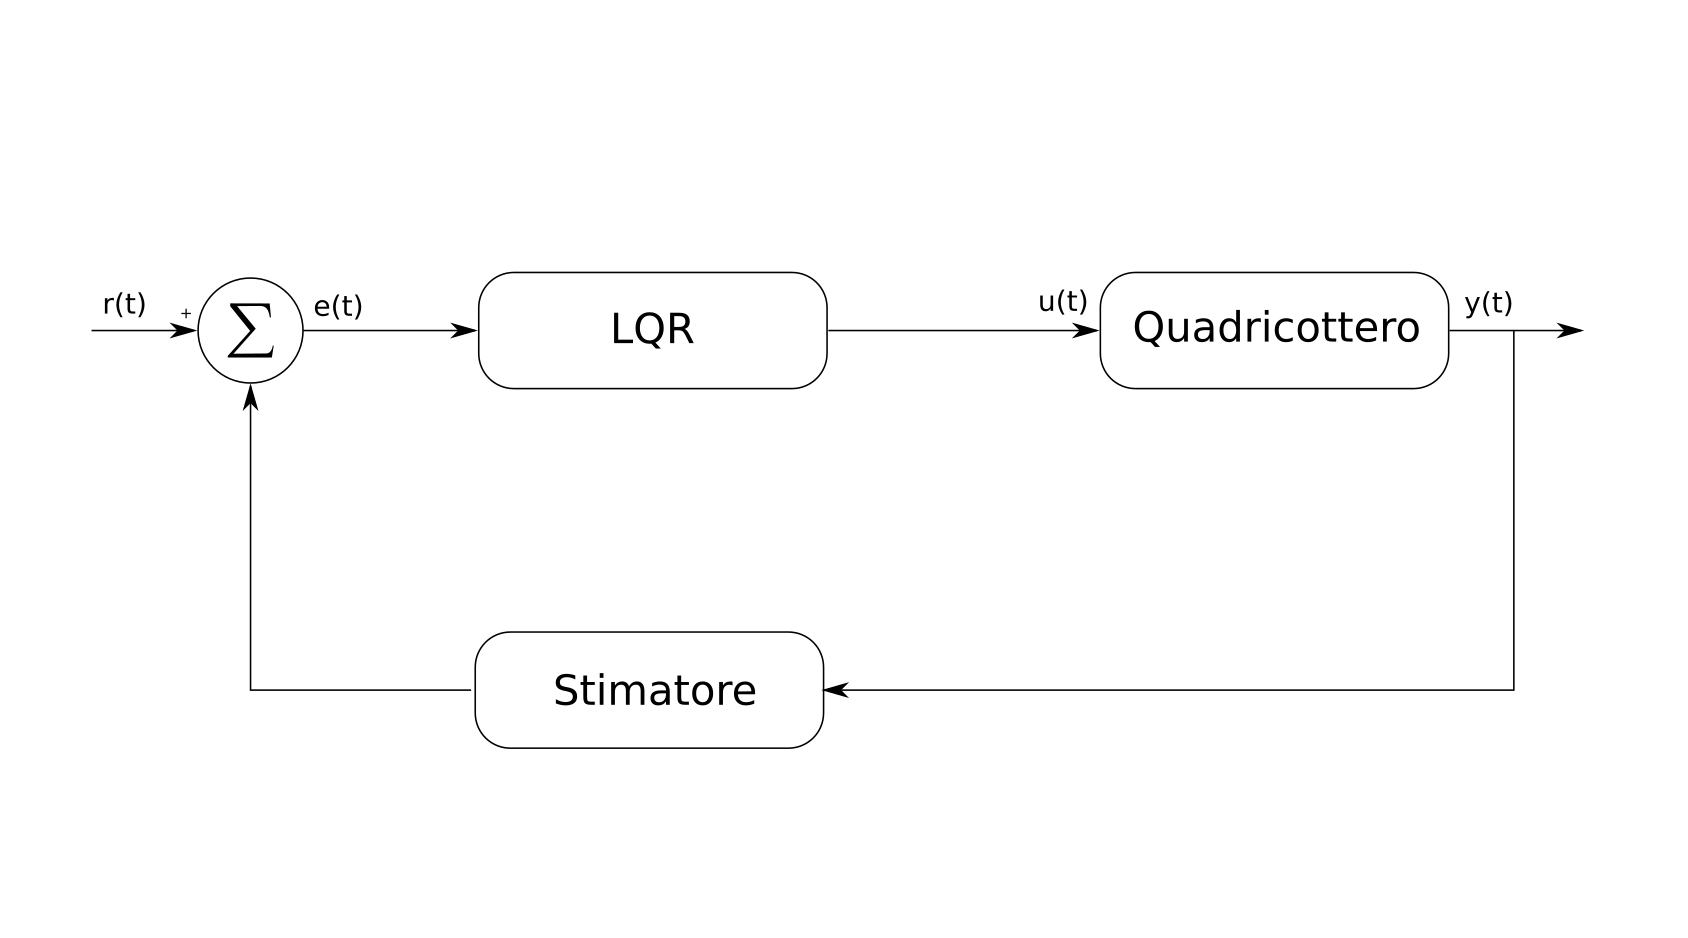
\includegraphics[width=0.6\textwidth]{SistemaQuadrirotore/Figure/LQR}
	\caption{Schema di applicazione del controllore LQR}
\end{figure}
 

\subsubsection{Controllore $H_\infty$}

Il controllore $H_\infty$ si ottiene esprimendo la soluzione del controllo attraverso una formulazione matematica, prende il nome dallo spazio matematico in cui ha luogo l'ottimizzazione, ovvero lo spazio di Hardy. Il problema principale di questo approccio è la complessità analitica che risiede nell'ottimizzazione stessa. Il sistema così trovato però ha il vantaggio di essere di più facile implementazione su sistemi multi-variabili. Facendo riferimento a \cite{GrimbleM.J1991Hrcd}, si utilizza la rappresentazione con funzioni di trasferimento e considerando anche la presenza di incertezza della modellazione, Eq (\ref{eq:SistemaQuadrirotore_G_inf_TF}).

\begin{equation}\label{eq:SistemaQuadrirotore_G_inf_TF}
	y(s) = \left(G_0(s) + \Delta G_A(s)\right) u(s) 
\end{equation}

Dove $y(s)$ è la trasformata di Laplace della risposta del sistema, $G_0(s)$ rappresenta la funzione di trasferimento del sistema nominale, $\Delta G_A(s)$ la funzione di trasferimento della perturbazione dovuta all'incertezza e $u(s)$ la trasformata di Laplace del comando.
Definendo $n(s)$ l'errore di misurazione e $r(s)$ il segnale di riferimento, si determina l'errore nominale di misurazione attraverso le equazioni (\ref{eq:SistemaQuadrirotore_G_inf_err_0}) e (\ref{eq:SistemaQuadrirotore_G_inf_z(s)}).

\begin{equation}\label{eq:SistemaQuadrirotore_G_inf_err_0}
	e_0(s) = r(s) -z(s)
\end{equation}

\begin{equation}\label{eq:SistemaQuadrirotore_G_inf_z(s)}
	z(s) = y(s) + n(s)
\end{equation}

Il comando si esprime utilizzando l'equazione (\ref{eq:SistemaQuadrirotore_G_inf_u(s)}).
\begin{equation}\label{eq:SistemaQuadrirotore_G_inf_u(s)}
	u(s) = C_0(s) e_0(s)
\end{equation}
Dove $C_0(s)$ è la funzione di trasferimento necessaria al controllo.
Si definiscono inoltre la funzione di trasferimento della sensibilità nominale e del suo complementare, Eq. (\ref{eq:SistemaQuadrirotore_G_inf_sens}), (\ref{eq:SistemaQuadrirotore_G_inf_compsens}), rispettivamente.

\begin{equation}\label{eq:SistemaQuadrirotore_G_inf_sens}
	S_0(s) = \frac{1}{1+ G_0(s) C_0(s)}
\end{equation}

\begin{equation}\label{eq:SistemaQuadrirotore_G_inf_compsens}
	T_0(s) = 1- S_0(s)
\end{equation}

Si definisce la norma infinita nello spazio di Hardy nell'equazione (\ref{eq:SistemaQuadrirotore_G_inf_Hardy}).
\begin{equation}\label{eq:SistemaQuadrirotore_G_inf_Hardy}
	\|(X(s)\|_\infty = \sup_\omega \mid X(j \omega) \mid
\end{equation}

Si applica infine la definizione (\ref{eq:SistemaQuadrirotore_G_inf_Hardy}) alla funzione $T_0(j \omega) B_w(\omega)$, dove $B_m(\omega)$ rappresenta il modulo della restrizione che si vuole imporre all'incertezza normalizzata $\frac{\Delta G_A(j \omega)}{G_0 (j \omega)}$ per una determinata frequenza, ottenendo l'equazione (\ref{eq:SistemaQuadrirotore_G_inf_maxim}).

\begin{equation}\label{eq:SistemaQuadrirotore_G_inf_maxim}
		\|T_0 B_m\|_\infty = \sup_\omega \mid T_0(j \omega) B_m(\omega) \mid
\end{equation}

Analogamente si studia l'effetto del disturbo ottenendo l'equazione (\ref{eq:SistemaQuadrirotore_G_inf_maximaS}. Attraverso la selezione della funzione $W_d(\omega)$ si enfatizza la regione di frequenze nella quale occorre aumentare la sensibilità per ridurre l'effetto dei disturbi esterni.

\begin{equation}\label{eq:SistemaQuadrirotore_G_inf_maximaS}
	\|S W_d\|_\infty = \sup_\omega \mid S(j \omega) W_d(\omega) \mid
\end{equation}
Dove 
\[ 
	S(j \omega) = \frac{1}{1+ \left[G_0(j \omega) + \Delta G_A((j \omega) \right]C_0(s)}
\]

Da queste due definizioni si definisce la funzione di costo, Eq. (\ref{eq:SistemaQuadrirotore_G_inf_Costo}), dalla quale selezionando scegliendo le funzioni $B_m$ e $W_d$ si ricava la funziona di trasferimento del controllore $C_0$.

\begin{equation}\label{eq:SistemaQuadrirotore_G_inf_Costo}
	J_\infty = \| S W_d \|_\infty + \| T B_m\|_\infty
\end{equation}

L'applicazione per il quadricottero di questo tipo di controllore e stata studiata in \cite{G_inf}.

\subsection{Controllori non lineari}

\subsubsection{Controllore con Feedback Linearization}

Questo tipo di controllore viene utilizzato comunemente quando è necessario controllare dei sistemi non lineari. La logica di funzionamento prevede di utilizzare un controllo lineare, introducendo una mappatura dell'ingresso al sistema, attuando di fatto un cambiamento delle variabili di controllo, in modo che il sistema di controllo lineare sia in grado di controllare il sistema non lineare.  Questo tipo di approccio ha lo svantaggio però di essere molto sensibile alle incertezze e i rumori dei sensori, fattore che ne inficia la robustezza \cite{KimJinho2020ACSo}.

Partendo da un sistema non lineare che è possibile modellare nella forma (\ref{eq:SistemaQuadrirotore_Sistemanonlin}), si ricava il sistema lineare (\ref{eq:SistemaQuadrirotore_Sistemalin}). Questa linearizzazione avviene attraverso l'introduzione di una mappatura del comando espressa dalla equazione (\ref{eq:SistemaQuadrirotore_FL_com}). Si utilizza quindo la nuova variabile di controllo $v$ in un classico sistema di controllo lineare. La determinazione delle matrici $\gamma(x)$ e $\psi(x)$ è quindi la chiave per rimuovere le linearità del sistema. Quando non risulta possibile determinare esattamente queste due matrici, si utilizza una approssimazione oppure una linearizzazione solamente parziale, \cite{IsidoriA2003NCS}.

\begin{equation}\label{eq:SistemaQuadrirotore_Sistemanonlin}
	\dot{x} = f(x) + G(x) u
\end{equation}

\begin{equation}\label{eq:SistemaQuadrirotore_Sistemalin}
	\dot{z} = A z + B v
\end{equation}

\begin{equation}\label{eq:SistemaQuadrirotore_FL_com}
	u = \gamma^{-1}(x) \left[- \psi(x)+v\right]
\end{equation}

\begin{figure}
	\centering
	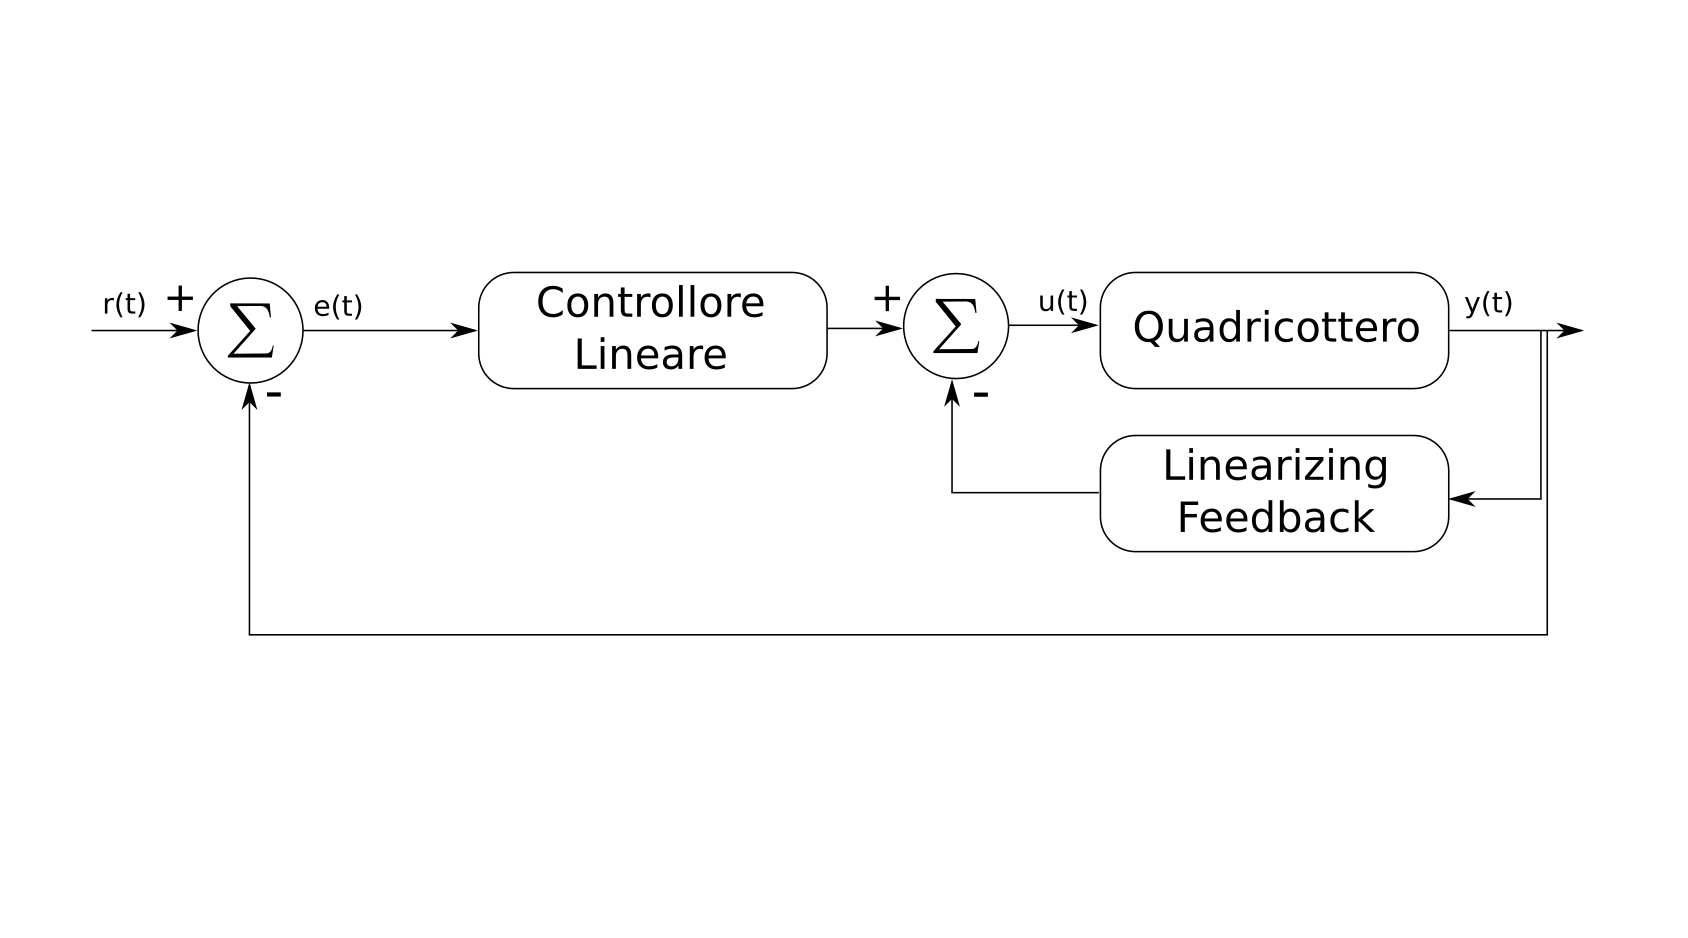
\includegraphics[width=0.6\textwidth]{SistemaQuadrirotore/Figure/FLP}
	\caption{Schema di applicazione del controllore con Feedback Linearization}
\end{figure}

Nella stessa pubblicazione, \cite{G_inf}, questo approccio di controllo viene utilizzato. Il closed-loop ottenuto attraverso la Feedback Linearization, viene controllato dal controllore $H_\infty$.

\subsubsection{Controllore con Backstepping}
La tecnica di Backstepping consiste nel suddividere il modello in sottoparti e stabilizzare in modo sequenziale i sottosistemi ottenuti.
Come esempio di implementazione di questi tipo di sistema di controllo si fa riferimento a \cite{Backstepping}, nella quale esprimendo il comando effettivamente applicato sui rotori $u = \left[\dot{F_1} ,\dot{F_2}, \dot{F_3},\dot{F_4} \right]$, si suddivide il sistema in tre sottosistemi, Eq. (\ref{eq:SistemaQuadrirotore_BACKSis}).

\begin{equation}\label{eq:SistemaQuadrirotore_BACKSis}
\begin{array}{r@{}l}
	S_1 &:
	\begin{cases}
	\dot{x_1} = x_2 \\ \dot{x_2} = f_0(x_2,x_3,x_5,x_6) + g_0(x_5,x_7)\varphi_0(x_3) \\ \dot{x_3}=x_4 \\ \dot{x_4} = f_1(x_3,x_4,x_6,x_7) + g_1(x_5,x_7)\varphi_1(x_7)
	\end{cases} \\ 
		S_2 &:
	\begin{cases}
	\dot{x_5} = x_6 \\ \dot{x_6} = f_2(x_3,x_4,x_6,x_7) + g_2(x_3) \varphi_2(x_7)
	\end{cases} \\
		S_3 &:
	\begin{cases}
	\dot{x_7}=u
	\end{cases}
\end{array}
\end{equation}
Dove :
\[
\begin{matrix}
x_1 = \begin{bmatrix}
x \\ y
\end{bmatrix}, &
x_3 = \begin{bmatrix}
\phi \\ \theta
\end{bmatrix}, &
x_5 = \begin{bmatrix}
\psi \\ z
\end{bmatrix}, \\
x_2 = \begin{bmatrix}
\dot{x} \\ \dot{y}
\end{bmatrix}, &
x_4 = \begin{bmatrix}
\dot{\phi} \\ \dot{\theta}
\end{bmatrix}, &
x_6 = \begin{bmatrix}
\dot{\psi} \\ \dot{z}
\end{bmatrix},
\end{matrix} \ 
x_7 = \begin{bmatrix}
F_1 \\ F_2 \\ F_3 \\ F_4
\end{bmatrix}.
\]
Le matrici $f_i$, $g_i$ e $\varphi_i$ sono ricavate attraverso la manipolazione del modello dinamico del quadricottero preso in considerazione.
L'obbiettivo è quello di stabilizzare il sistema complessivo. Si determinano quindi le misure di errore introducendo l'effetto di un controllo, Eq. (\ref{eq:SistemaQuadrirotore-BACKERR}), in modo da stabilizzare la soluzione del sottosistema utilizzando il criterio di Lyapunov. 

\begin{equation}\label{eq:SistemaQuadrirotore-BACKERR}
	\begin{array}{r@{}l}
		z_1 & = x_{1r} -x_1 \\
		z_2 & = x_2 - \dot{x_{1r}} - \alpha_1 z_1 \\
		z_3 & = x_{3r} - x_3 \\
		z_4 & = x_4 - x_{3r} - \alpha_3 z_3 \\
		z_5 & = x_{5r} -x_5 \\
		z_6 & = x_6 - x_{5r} - \alpha_5 z_5 \\
		z_7 &= x_{7r} - x_7 \\
		z_8 &= x_8 - \dot{x_{7r}} - \alpha_7 z_7
	\end{array}
\end{equation}

Le funzioni selezionate per questo controllo devo quindi soddisfare il criterio di Lyapunov. Si sceglie una funzione scalare $V(x,t)$ con argomento lo stato del sistema e con derivata prima continua. La funzione scelta deve soddisfare le seguenti tre condizioni:
\begin{itemize}
	\item $V(x,t)$ deve essere definita positiva
	\item $\dot{V(x,t)}$ deve essere definita negativa
	\item Per $V(x,t)$ che tende ad infinito $\mid{x}$ deve tendere all'infinito
\end{itemize}
Se queste condizioni sono soddisfatte allora la funzione scelta rispetta l'equilibrio nell'origine della superficie e si può dimostrare che questo equilibrio e globalmente asintoticamente stabile \cite{DesTestCarm}.

Un approccio simile viene utilizzato anche in \cite{Backstepping1}, nella quale viene messo in confronto questa tecnica di modellazione del controllore con il controllore SMC.

\subsubsection{Controllore Sliding Mode Control (SMC)}

Questo tipo di controllo prevede di utilizzare un segnale di comando discontinuo. Questo sistema risulta essere molto preciso e robusto, come verrà mostrato nelle simulazioni successive. A causa della discontinuità introdotta si può  osservare il fenomeno di chattering, che ha come effetto secondario l'aumento dell'utilizzo degli attuatori, ovvero un maggior consumo di batteria. Questo effetto può essere mediato applicando alcuni filtri in uscita dal controllore, che mediano le discontinuità \cite{KimJinho2020ACSo}. Il controllo basa il funzionamento sulla definizione di una superfice di sliding definita dallo stato del sistema, una volta portato su questa superficie attraverso il segnale discontinuo il controllore mantiene le oscillazioni nei dintorni di questa \cite{DesTestCarm}. Questo tipo di controllore è molto robusto e si comporta bene in presenza di rumore ed incertezze come l'effetto suolo.

Partendo dalla scrittura nella forma espressa nell'equazione (\ref{eq:SistemaQuadrirotore_SMC_sistema}), si considera una generica superficie $S(t) 0 \{ s(x,t) \in \mathbb{R}^n  \mid s(x,t) = 0\}$.
\begin{equation}\label{eq:SistemaQuadrirotore_SMC_sistema}
	\dot{x(t)} = f(x,t) +g(x,t) u(x,t)
\end{equation}

La funzione che definisce il controllo viene espressa introducendo una discontinuità in $s(x,t)=0$, Eq. (\ref{eq:SistemaQuadrirotore_SMC_comando}).
\begin{equation}\label{eq:SistemaQuadrirotore_SMC_comando}
	u(x,t) = \begin{cases}
		u^+ \ \text{Se} \ s(x,t) > 0 \\
		u^- \ \text{Se} \ s(x,t) < 0
	\end{cases}
\end{equation}

Imponendo che valga la condizione (\ref{eq:SistemaQuadrirotore_SMC_cond}), si definisce quindi il funzionamento in sliding mode.

\begin{equation}\label{eq:SistemaQuadrirotore_SMC_cond}
	s(x,t) \dot{s(x,t)} < 0
\end{equation}

Il funzionamento di questo controllore prevede due fasi nella sua attuazione. Una prima fase nella quale partendo da una condizione generica il sistema controllato tende a raggiungere la superficie di intersezione. La seconda fase in cui il sistema attua lo scivolamento lungo questa superficie oscillando attorno alla condizione di equilibrio, come mostrato in Figura (\ref{fig:SMC}).

\begin{figure}
	\centering
	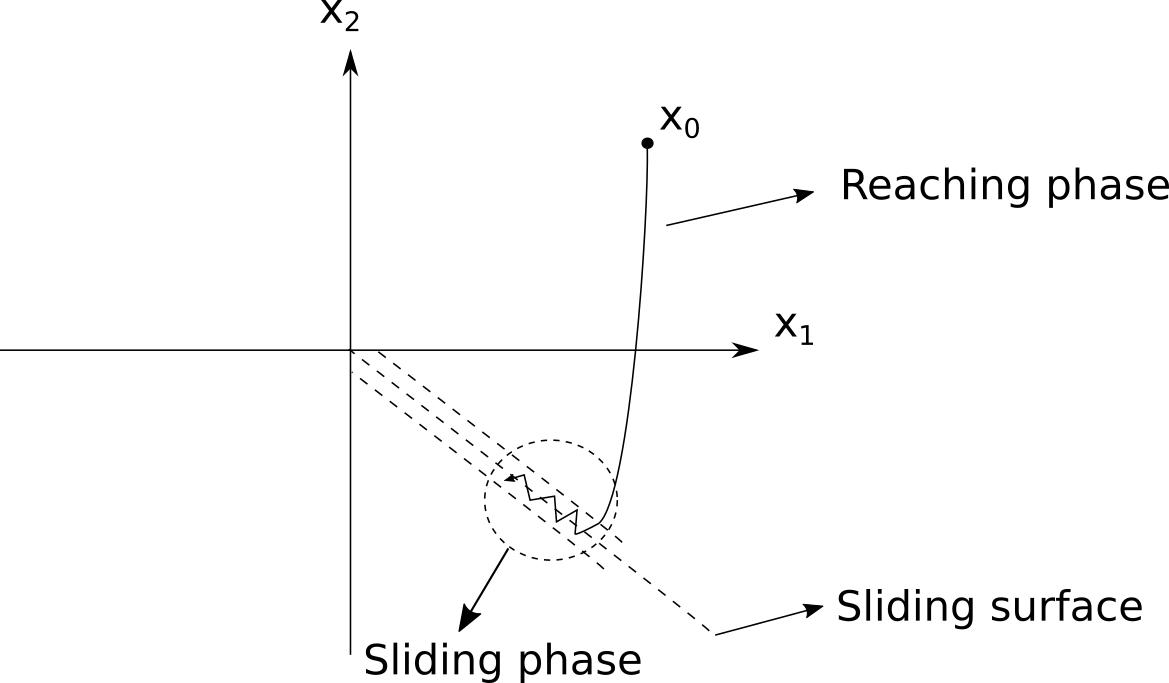
\includegraphics[width=0.6\textwidth]{SistemaQuadrirotore/Figure/SMC_fasi}
	\caption{Fasi di azionamento del controllore SMC \cite{LiShihua2017AiVS}}
	\label{fig:SMC}
\end{figure}

\begin{figure}
	\centering
	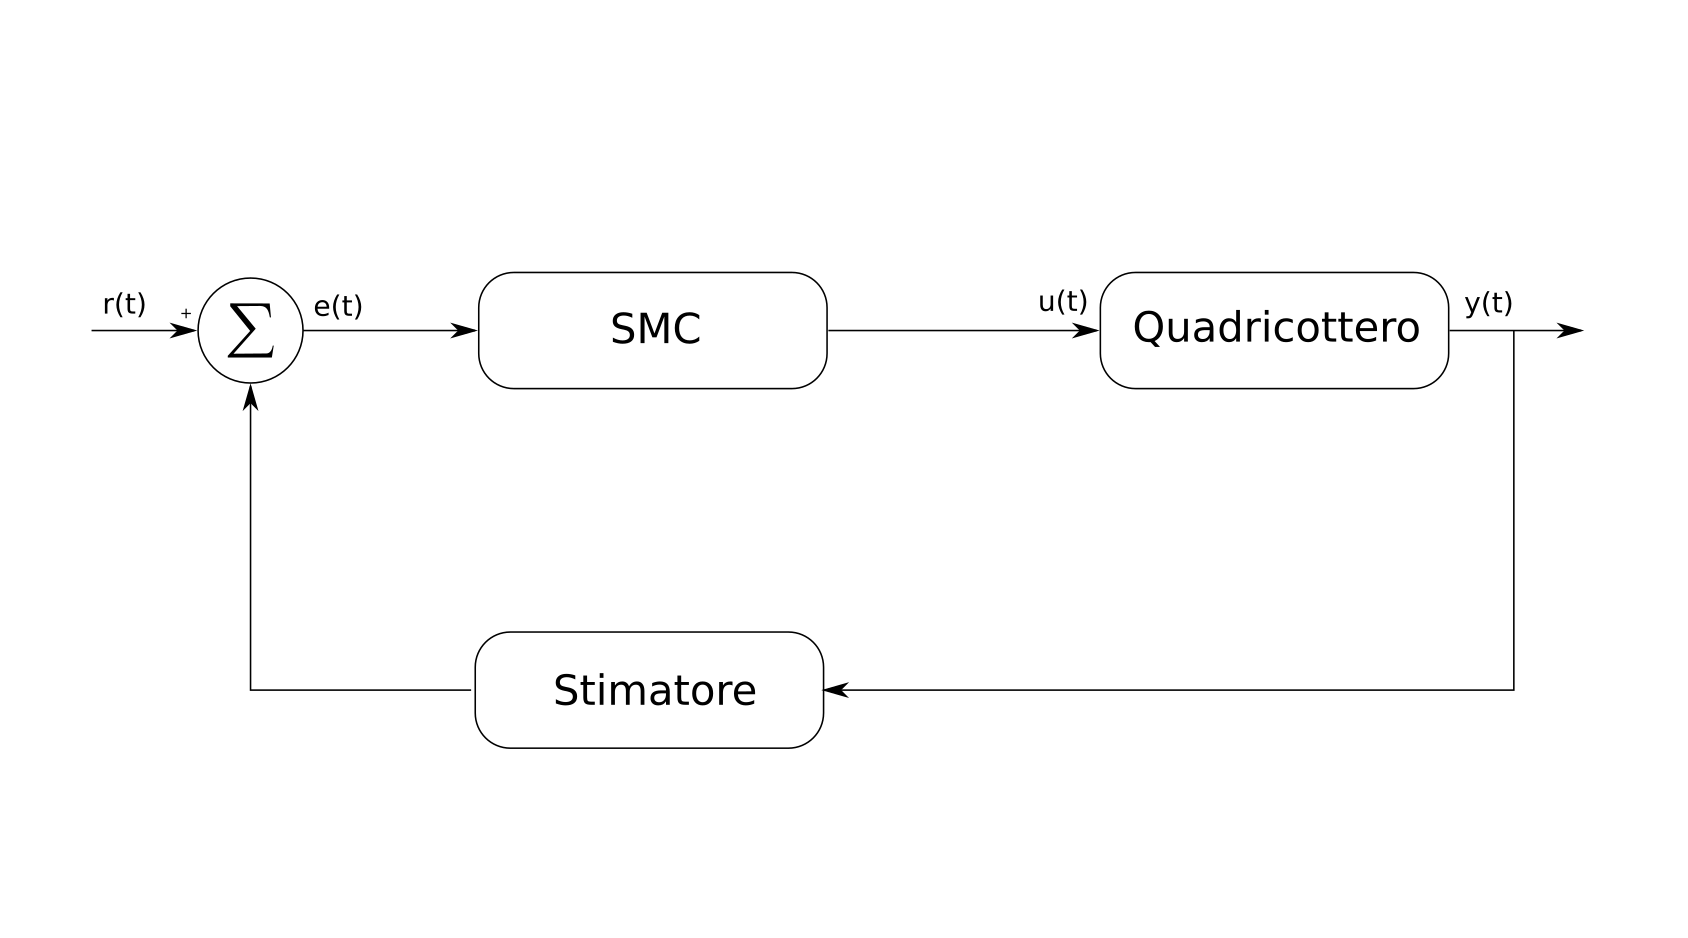
\includegraphics[width=0.6\textwidth]{SistemaQuadrirotore/Figure/SMC}
	\caption{Schema di applicazione del controllore SMC}
\end{figure}

\subsection{Controllori intelligenti}

\subsubsection{Controllore con Modello predittivo (MPC)}

Questo tipo di controllo si basa sulla previsione dello stato e del comando che verrà attuato seguendo dei modelli previsionali e stimatori. Molto utile se si vuole evitare di superare alcune imposizioni specifiche, per esempio le limitazioni in termini di capacità di attuazione o minimizzazione di funzioni di costo.
Per un controllo efficacie è necessario stimare il più precisamente possibile lo stato del velivolo, \cite{KimJinho2020ACSo}.


Il controllore basa il suo funzionamento su un rappresentazione discreta nel tempo. Dato quindi un segnale $s(t)$ da inseguire, il controllore lo campiona in una sequenza di punti. Si utilizza una seconda traiettoria di riferimento $y(k)$ che descrive l'andamento che il quadritotore deve seguire per raggiunge la sequenza di punti impostati nei sotto intervalli osservati. Un aspetto critico è la selezione della funzione da utilizzare come riferimento per inserire il controllore in closed-loop, una possibile scelta ricade nel segnale di riferimento esponenziale \cite{AbdolhosseiniM2013AEMP}. Partendo quindi dalla sequenza di punti di riferimento, applicando un modello predittivo in una finestra di tempo discreta si determina il comando che permette di inseguire la seconda traiettoria scelta. Facendo scorrere per ogni interazione la finestra temporale utilizzata e il campionamento su di essa si implementa questo tipo di controllo, determinando passo-passo in comando.
Per ottimizzare ila soluzione e determinare il segnale di attuazione ad ogni interazione in \cite{AbdolhosseiniM2013AEMP}, viene proposta l'ottimizzazione sull'errore, Eq. (\ref{eq:SistemaQuadrirotore_MPC_ERR}).
\begin{equation}\label{eq:SistemaQuadrirotore_MPC_ERR}
	\sum_{1}^{i} \left[r(k+1 \mid k) - \hat{y}(k+i \mid k)\right]^2
\end{equation}

Dove $\hat{y}$ rappresenta l'output misurato e $r$ il segnale di riferimento generato attraverso questo approccio di controllo.

\begin{figure}
	\centering
	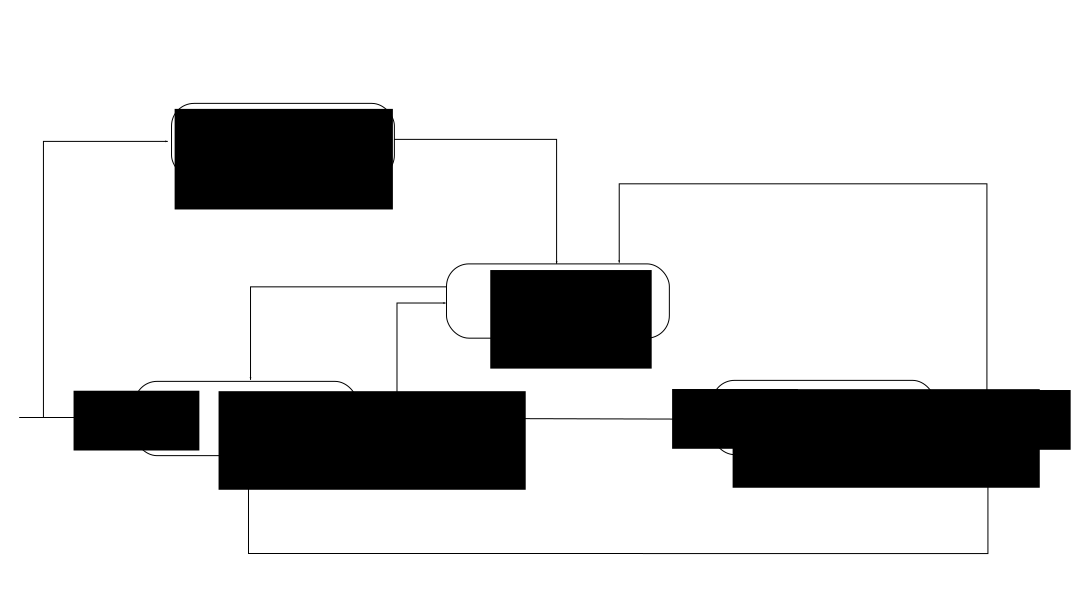
\includegraphics[width=0.6\textwidth]{SistemaQuadrirotore/Figure/MPC}
	\caption{Schema di applicazione del controllore MPC}
\end{figure}

\subsubsection{Controllore con logica Fuzzy}

Il sistam di controllo Fuzzy è fondamentalmente composto da tre parti principali: l'unità che si occupa della fuzzification, l'unità che determina le regole da implementare e l'uotput del controllo e infine il componente che determina dallo stato dell'output il segnale del controllo. 
L'implementazione delle regole prevede di utilizzare degli stati logici non binari, compresi tra 0 e 1. Applicando questo concetto alla misura dell'errore, si determina una classificazione in funzione all'appartenenza di questo ad una determina condizione, per esempio : nullo, piccolo negativo, medio positivo, ecc. Nel cuore del controllore, utilizzando le proprietà matematiche dei set logici cosi definiti, si descrivono quindi le regole di esecuzione in base agli ingressi logici. Il risultato di questo processo di applicazione delle regole porta a definire un analogo set logico di uscita. attraverso l'unità di defuzzification, utilizzando gli stati logici di uscita si determina il segnale di comando da impartire al sistema governato, \cite{introFuzzy}.
Lo stesso tipo di approccio può

Nella publicazione \cite{introFuzzy} il sistema fuzzy viene utilizzato per controllora l'assetto del drone.

\begin{figure}
	\centering
	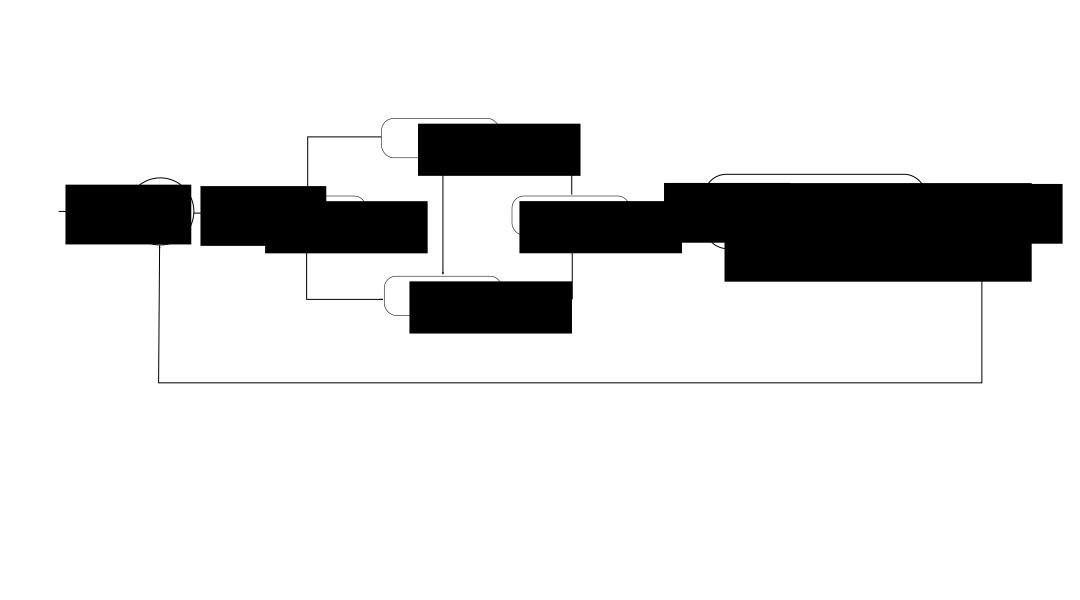
\includegraphics[width=0.8\textwidth]{SistemaQuadrirotore/Figure/Fuzzy}
	\caption{Schema di applicazione del controllore Fuzzy}
\end{figure}

\subsubsection{Controllore con Neural Network}

Si utilizza una rete neurale formata da diversi layer con la quale attraverso una fase di addestramento si ottiene un sistema di controllo. La rete è formata da neuroni collegati attraverso dei collegamenti pesati. Il vantaggio di questo metodo di controllo è la capacità di avere risultati migliori rispetto ai normali controlli lineari senza dover necessariamente conoscere la dinamica del quadrirotore e i suoi parametri.

\begin{figure}
	\centering
	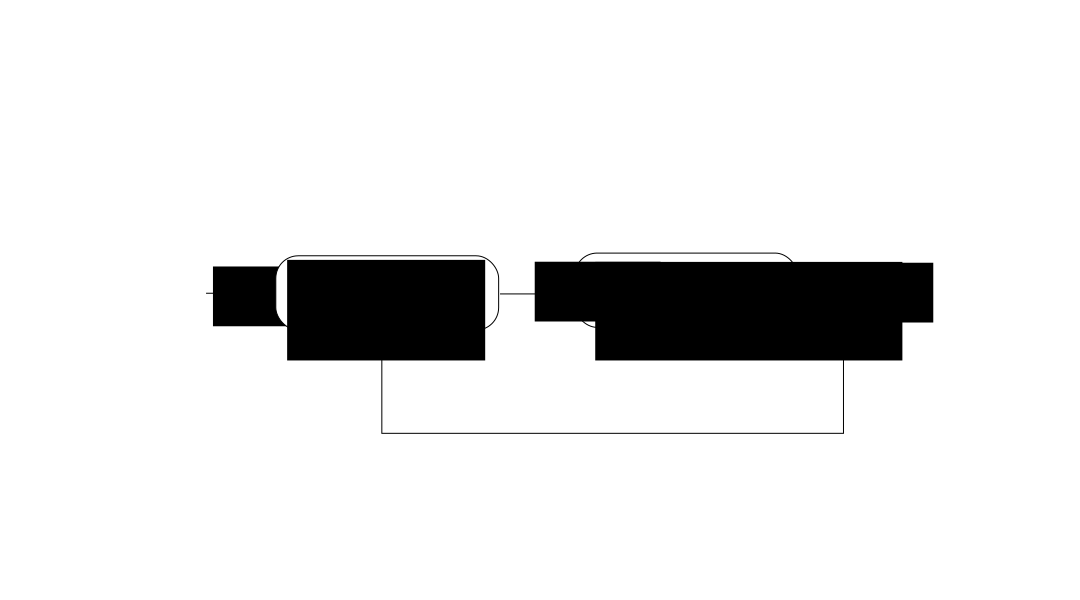
\includegraphics[width=0.6\textwidth]{SistemaQuadrirotore/Figure/NN}
	\caption{Schema di applicazione del controllore con Neural Network}
\end{figure}
